\chapter{Datos y metodología}
\label{chapter:datos_metodologia}

\section{Datos: La Encuesta Financiera de las Familias}\label{section:datos}

Para este proyecto se van a utilizar los datos de la Encuesta Financiera de las Familias (EFF). La EFF es una encuesta oficial a hogares elaborada por el Banco de España y está incluida en el Plan Estadístico Nacional. Su primera edicion se realizó en el año 2002, y se ha producido de manera trienal hasta el año 2020. Desde entonces, se produce de manera bienal.

El objetivo de la EFF es recabar información sobre las condiciones financieras de los hogares residentes en España. Su cuestionario principal está compuesto por nueve secciones. Las secciones 1 y 6 recogen información sociodemográfica individualizada de todos los miembros del hogar y también información individualizada sobre la situación laboral y los ingresos de cada miembro del hogar mayor de 16 años. El resto de secciones recogen información detallada sobre los activos, deudas, gastos y uso de medios de pago del hogar en su conjunto, y contienen módulos específicos que recogen información individualizada de ciertos elementos patrimoniales si el hogar los posee, como propiedades inmobiliarias, negocios gestionados por cuenta propia o planes de pensiones. Los hogares formados por más miembros mayores de edad y que posean más elementos patrimoniales responderán a más preguntas. Por poner un ejemplo con números, en la EFF2017 a cada hogar se le plantearon entre 137 y 594 preguntas, siendo la mediana de 259 preguntas (\cite{effmethod2017}).

La EFF es la única fuente estadística que permite relacionar información sobre activos, deudas, ingresos y gastos de los hogares españoles. Esto permite analizar las decisiones de inversión y financiación de las familias y conocer su situación patrimonial, y gracias a ello tener un mayor conocimiento de la economía española y poder utilizarlo para hacer un diseño adecuado de politicas públicas. Por nombrar algunos ejemplos de estudios realizados con la EFF, se ha utilizado para cuantificar el ahorro adicional generado para los partícipes en planes de pensiones de empresa (\cite{gomez2022pensiones}), para caracterizar cómo afectó la pandemia del Covid-19 a la situación patrimonial de los trabajadores más afectados por dicha crisis (\cite{alvargonzalez2020pandemia} o para analizar las diferencias en aceptación y uso de tarjetas de crédito y banca online entre diferentes grupos de hogares desde el año 2002 (\cite{crespo2023bancaonline}).

El diseño de la muestra de la EFF tiene dos características importantes: un sobremuestreo de hogares ricos y un componente longitudinal o panel. El sobremuestreo de ricos\footnote{La muestra de la EFF es seleccionada por el Instituto Nacional de Estadística, en colaboración con la Agencia Tributaria, a partir de las declaraciones individuales más recientes en el Impuesto sobre el Patrimonio. Para una descripción más detallada del proceso, puede consultarse \cite{effmethod2017}.} garantiza poder analizar con suficiente precisión el comportamiento de los hogares de la parte alta de la distribución de riqueza. Este detalle es importante porque la distribución de la riqueza entre los hogares es asimétrica, por lo que sólo unos pocos hogares, especialmente los más ricos, son los que invierten en ciertos activos. Posteriormente, para poder hacer análisis válidos para la población española, a cada hogar se le asigna un peso muestral que indica a cuántos hogares de la población española representa ese hogar\footnote{Para más detalle sobre el cálculo de los pesos muestrales, consultar \cite{effmethod2002}.}. Por otro lado, el compomente panel indica que se vuelve a entrevistar a hogares que participaron en ediciones anteriores. Esto permite monitorearles durante períodos de hasta diez años, y observar los cambios en las variables de interés de la encuesta. El número máximo de ediciones en las que un hogar puede participar en la EFF es de cuatro olas consecutivas. Si cesa su participación antes de completar sus cuatro ediciones, se descarta de la muestra y no vuelve a ser contactado en olas posteriores. Finalmente, para sustituir a los hogares descartados del panel rotatorio y mantener la representatividad de la muestra, en cada nueva ola de la EFF se añade una nueva muestra de refresco a la muestra panel.

Volviendo a los datos, en este proyecto se utiliza información que proviene tanto de las respuestas al cuestionario de la EFF, como del paradata recopilado durante la producción de los datos. Es importante conocer las etapas de este proceso de producción para poder entender los datos. En la figura 4.1. puede observarse un resumen de este proceso. La producción de la EFF se divide en dos grandes fases: Campo y Post-Campo. Durante el Campo se contacta con los hogares, se realizan las entrevistas personales, se procesan los datos y se realiza parte de la revisión de los mismos. En el Post-Campo se termina el proceso de revisión, se evalúa el grado de no-respuesta de los datos de cada hogar para eliminar las entrevistas con poco contenido informativo, y se procede a la imputación de la no-respuesta. Tras este último proceso, se obtienen los datos finales.

\begin{figure}[ht]
	\centering
	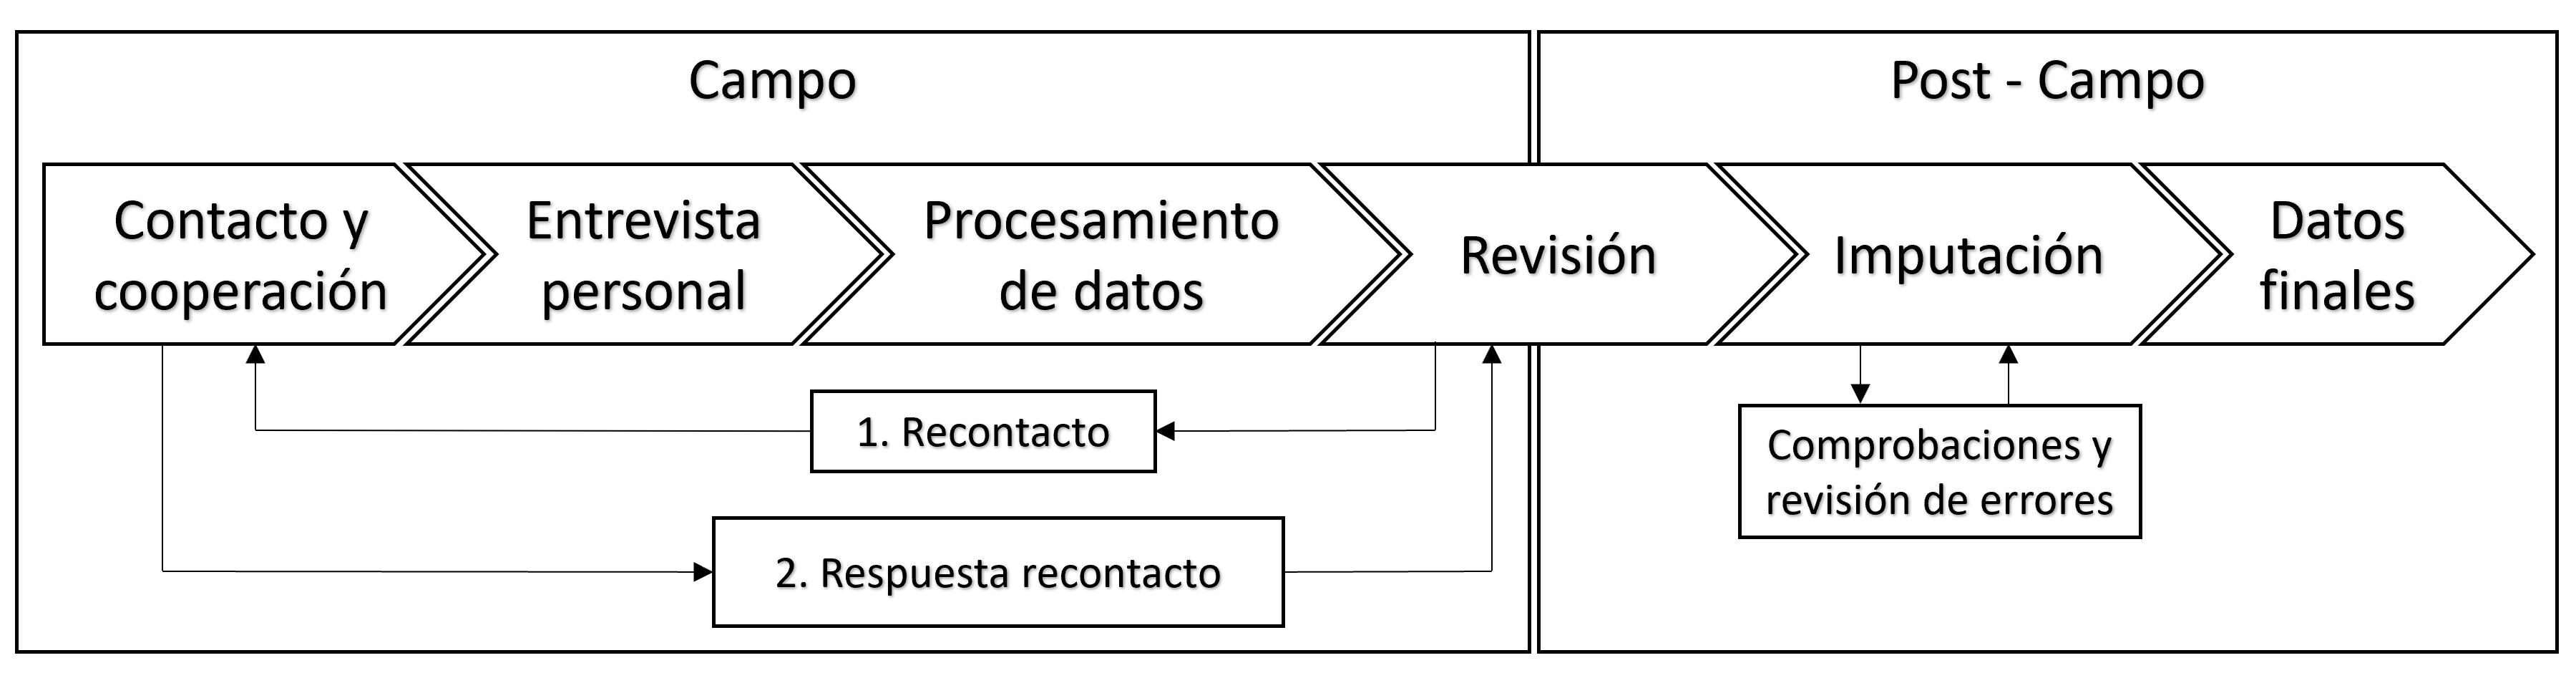
\includegraphics[width=1\textwidth]{figs/fases_creacion_datos_eff.png}
	\caption{Fases de la creación de datos de la EFF}
	\label{fig:eff_phases}
\end{figure}

A continuación se hace una breve descripción de los aspectos más relevantes de las subfases y que son importantes para la selección de variables para este estudio.

\begin{itemize}
    \item \textbf{Contacto y cooperación:} Se envía una carta a los hogares para informar sobre su selección para la encuesta y que una persona les visitará personalmente en su domicilio para hacerles una entrevista personal. El contacto puede requerir varias visitas, ya que es necesario que algún miembro del hogar esté físicamente en su hogar cuando tenga lugar la visita presencial. La información sobre cada intento (fecha y hora, resultado...) se recoge en un ordenador. Antes de establecer el contacto, los entrevistadores rellenan un cuestionario que recoge información sobre las características del barrio y del edificio en el que vive el hogar. Los entrevistadores también llevan documentación sobre la encuesta que pueden utilizar para intentar convencer al hogar, como por ejemplo un folleto con noticias de prensa en las que se ha hablado de la EFF.
    \item \textbf{Entrevista personal:} Se realiza una entrevista personal a la persona con más conocimiento de las finanzas del hogar, que se denomina Persona de Referencia o PR. La PR puede ser miembro del hogar, o un representante del mismo, demoninado proxy, siempre y cuando sea la persona con mayor conocimiento de las finanzas del hogar. También pueden participar otros miembros del hogar. Las entrevistas suelen durar entre una hora y hora y media (\cite{effmethod2017}). Antes de empezar la entrevista, se pide a la PR su consentimiento para que algunas partes de la misma puedan ser grabadas en audio por motivos de calidad de los datos. La entrevista puede realizarse aunque no haya grabación. Los entrevistadores recogen las respuestas en un ordenador o una tablet (CAPI), y también pueden anotar en comentarios de texto todos los detalles que consideren importantes para la revisión. La PR puede decidir no contestar a ciertas preguntas. Su valor se asignará como missing, y se imputará más adelante. Las cantidades monetarias pueden responderse en valor puntual, o dentro de un rango de valores. Tras la entrevista, y sin la presencia de los hogares, los entrevistadores rellenan un cuestionario con información sobre el desarrollo de la entrevista, en el que por ejemplo se recoge el nivel de comprensión de la PR a las preguntas, el nivel de interés mostrado por la PR o cuántas personas han participado en la entrevista.
    \item \textbf{Procesamiento de datos:} Los ordenadores y servidores de la empresa de campo procesan los datos recogidos durante el contacto con los hogares y durante las entrevistas. Se crean tres ficheros, uno con las respuestas al cuestionario, uno con la información de los contactos con cada hogar, y finalmente uno con la información del paradata recogido por el ordenador durante la entrevista\footnote{También se crea un fichero con los comentarios de texto recogidos por los entrevistadores durante la entrevista, pero no se ha podido incluir en este estudio por falta de tiempo.}.
    \item \textbf{Revisión:} Un equipo de personas revisa individualmente todas las entrevistas y corrige los errores que puedan detectarse. Si hay información relevante que se ha recogido erróneamente o se ha omitido, se contacta de nuevo con el hogar para corregirlo o recuperar esa información. Este recontacto se hace por teléfono. Toda la información sobre la revisión (cambios sobre variables, recontactos...) se recoge en una aplicación informática y puede ser exportada en ficheros de diversos formatos (csv, excel...).
    \item \textbf{Imputación:} Se analiza la proporción de preguntas sin responder dentro de cada entrevista (no-respuesta), y se eliminan las que no superen ciertos umbrales de calidad. Todas las variables que contienen no-respuesta se imputan mediante técnicas de imputación múltiple\footnote{Los métodos de imputación múltiple utilizados en la EFF pueden consultarse en \cite{barcelo2006imputation}.}. Se crean 5 ficheros con datos imputados.
\end{itemize}

Con respecto a los procedimientos de Contacto y Entrevista personal, es necesario mencionar que algunos elementos tuvieron que modificarse durante la EFF2020, ya que el campo tuvo lugar entre noviembre de 2020 y junio de 2021, y se vió afectado por la pandemia del Covid-19. Durante esa ola, los entrevistadores siguieron visitando personalmente a los hogares para conseguir su colaboración\footnote{Durante el principio del campo, algunos hogares panel fueron contactados sólo por teléfono, pero a las pocas semanas se decidió establecer la visita personal como el procedimiento estándar.}, pero siempre respetando las medidas de distanciamiento social. Las entrevistas se realizaron de manera telefónica asistida por una tablet (CATI). El resto de procedimientos se mantuvieron como en otras ediciones.

Para la elaboración de este proyecto se utiliza la información recopilada durante las olas de la EFF2017, EFF2020 y EFF2022 \footnote{En el momento de escribir este documento, la EFF2022 se encontraba en pleno proceso de imputación, por lo que el equipo del Banco de España ya conocía los resultados de participación de esa ola y era posible utilizarlos para este proyecto.}. Estas ediciones son las únicas que cuentan con la información más detallada de paradata y de las características de los entrevistadores. En ediciones anteriores esta información o no está disponible, o contiene errores de medida que no son fácilmente corregibles. A pesar de esto, es posible identificar en cuántas ediciones ha participado cada hogar, por lo que es posible utilizar información que se remonta hasta la edición de la EFF2011. Los ficheros de datos que se utilizan durante este proyecto son:

\begin{itemize}
    \item \textbf{Fichero de trabajo:} Registro de hogares con entrevistas válidas. Hay uno para cada edición de la encuesta. Contiene la información de las respuestas de los hogares, incluyendo las correcciones y ediciones de la revisión. Se indican los datos que deben ser imputados. También incluye variables auxiliares generadas para el proceso de imputación (características del hogar, de los miembros, del municipio...) y contadores de no respuesta de cada entrevista. Es el fichero que se utiliza para imputar. Se utilizan dos ficheros, el de la EFF2017 y el de la EFF2020.
    \item \textbf{Fichero de datos imputados:} Registro de hogares que contiene las respuestas al cuestionario después de haber imputado los datos con no-respuesta de los hogares. Hay cinco ficheros para cada edición, pero por simplicidad sólo se utiliza uno de los conjuntos de datos de la imputación multiple. Sólo contiene variables imputadas e indicadores de las características del hogar. Se utilizan dos ficheros, los de EFF2017 y EFF2020.
    \item \textbf{Fichero de contactos:} Registo de hogares contactados durante una ola de la EFF. Hay uno para cada ola de la EFF. Contiene información sobre el número de intentos de contacto con cada hogar, la fecha en que se produjo, el resultado de cada uno de ellos (aplazamientos, rechazos...) y las respuestas al cuestionario de vecindario rellenado por los entrevistadores. Se utilizan tres ficheros, los de EFF2017, EFF2020 y EFF2022.
    \item \textbf{Fichero de revisión:} Registro de incidencias durante el proceso de revisión y los recontactos. hay uno para cada edición de la EFF. Contiene información general sobre el proceso de revisión (por ejemplo, si se ha realizado un recontacto), y el resto de registros son incidencias en los datos que se detectado (por ejemplo, si se ha omitido una propiedad inmobiliaria, se abrirá un registro indicando esa incidencia y cómo se ha solucionado). Se utilizan dos ficheros, los de EFF2017 y EFF2020.
    \item \textbf{Fichero de paradata:} Registro de las pantallas visualizadas durante el uso del software CAPI durante cada entrevista. Hay uno para cada edición de la EFF. Cada registro es una pantalla visualizada durante una entrevistacada entrevista y se recoge cómo fue la interacción del entrevistador con el ordenador en esa pantalla durante la entrevista. En concreto, contiene la fecha y hora en la que se cargó la pantalla, si se pasó a la pantalla siguiente (se dió una respuesta), el tiempo que se estuvo visualizando dicha pantalla, si se volvió a la pantalla anterior o incluso si se seleccionó parar la entrevista en esa pantalla. Si en una entrevista se pasó varias veces por una pantalla, esa pantalla tendrá tantos registros como veces se cargó esa pantalla. Es posible agrupar los registros por entrevista, pregunta o sección, y ver el flujo de pantallas que se siguió durante la entrevista. Se utilizan dos ficheros, los de EFF2017 y EFF2020.
    \item \textbf{Censo de entrevistadores:} Registro de entrevistadores que contiene la información disponible sobre los entrevistadores que han participado desde la EFF2014 a la EFF2022. Sólo hay un fichero.
\end{itemize}

\section{Metodología}
\label{section:method}

Tomando como referencia las estrategias de investigación propuestas en \cite{oates2022researching}, en este proyecto se presenta un 'Caso de estudio'. Se busca tener un conocimiento profundo sobre la participación de los hogares panel en el caso específico de la EFF, y buscar un modelo para predecirla.

La metodología de este proyecto se fundamenta en cuatro pilares. En primer lugar, en la recopilación de los datos de las entrevistas y los entrevistadores que participaron en las olas EFF2017, EFF2020 y EFF2022. El segundo pilar es la realización de un análisis descriptivo de un conjunto de variables con potencial para explicar la Attrition. En tercer lugar, en el entrenamiento de varios modelos basados en métodos de machine learning con datos de la EFF2017 y la EFF2020, y evaluar su rendimiento para predecir la participación de los hogares panel en la EFF2022. Para este ejercicio se adapta la implementación hecha en \cite{beste2023case} al caso de la EFF. Finalmente, se realiza una valoración de los resultados obtenidos y qué pasos podrían darse en el futuro para seguir desarrollando este proyecto.

El tratamiento de datos y el análisis descriptivo en este proyecto se ha realizado con lenguaje Python (3.8.8), y los paquetes scikit-learn (1.2.2, \cite{pedregosa2011scikit}), imbalanced-learn (0.10.1, \cite{lemaavztre2017imbalanced}) y xgboost (1.5.2, \cite{chen2016xgboost}) para la construcción de los modelos de machine learning.

El resto de esta sección se divide en tres apartados. Es primer lugar se da una breve descripción del proceso de recopilación de los datos y el análisis descriptivo. En el siguiente apartado se define la variable dependiente $Attrition$ y también las variables que se van a utilizar como predictores de los modelos. Finalmente, se cierra este capítulo con la descripción de la estrategia de entrenamiento y validación de los modelos.

\subsection*{Recopilación de datos y análisis descriptivo}

En este proyecto hay que vincular información de doce ficheros de datos. La vinculación se realiza a través de dos identificadores, uno a nivel de hogar y otro a nivel de entrevistador. Cada hogar que participa en una ola concreta de la EFF tiene un identificador único para esa edición, y ese identificador es común para todos los ficheros de datos generados durante esa edición. Esto permite vincular los datos del mismo hogar entre los diferentes ficheros de datos de una edición. Además, si ese hogar es panelista, los ficheros de trabajo, datos imputados y contactos también incluyen el identificador único que tiene ese hogar en la ola anterior. Esto permite hacer la vinculación con la información de ese hogar recogida en ediciones anteriores de la EFF.

Por otro lado, la vinculación con la información del censo de entrevistadores se realiza a través de un identificador único que tiene cada entrevistador y que permanece inalterable a lo largo de las olas. Este indicador aparece como una variable adicional en el fichero de trabajo de cada ola, por lo que es posible identificar a la persona que realizó cada entrevista en cada una de las olas en las que participó. Esto además permite vincular los ficheros de hogares con los de entrevistadores.

Para realizar el análisis descriptivo, se han realizado tres tipos de tareas:
\begin{enumerate}[noitemsep]
    \item Exploración de las estructuras de datos de los ficheros. Esto ha permitido identificar los diferentes tipos de registros y la cantidad, tipología y codificación de las variables.
    \item Análisis de distribuciones individuales de todas las variables mediante cálculos de estadísticos descriptivos y representaciones visuales mediante histogramas y gráficos box-plot para las variables numéricas, y gráficos de columnas para las variables categóricas.
    \item Análisis de las relaciones entre las variables, y de manera particular con el Panel Attrition. Para analizar la relación entre variables continuas se han utilizado printipalmente gráficos de nubes de puntos y se han calculado los coeficientes de correlación entre cada variable numérica. Las relaciones entre variables categóricas se han realizado mediante el uso de gráficos de columnas, gráficos de mekko y test de independencia chi-cuadrado. Finalmente, la relación entre variables categóricas y numéricas se ha realizado visualmente con histogramas y box-plots de las variables continuas para cada categoría, y un análisis ANOVA en los casos que se cumplían los supuestos para este análisis.
\end{enumerate}

\subsection*{Variable \textit{Attrition} y predictores}

El objetivo del estudio es encontrar un modelo para predecir si un hogar que ha participado en la ola $t$ de la EFF no volverá a participar en la siguiente ola $t+1$. Para ello, se define la variable \textit{Attrition} como una variable dicotómica que toma valor 0 si el hogar vuelve a participar, y valor 1 si no vuelve a participar:

\begin{equation}
Attrition =
  \begin{cases}
    0       & \quad \text{el hogar participa en la ola $t+1$} \\
    1  & \quad \text{el hogar no participa en la ola $t+1$}
  \end{cases}
\end{equation}

En el cuadro \ref{table:attrition} puede observarse que, en las olas de 2020 y 2022, la mayoría de los hogares panel volvieron a participar. Esto provoca un ligero desbalance entre las observaciones de cada clase de Attrition, y durante los primeros entrenamientos y evaluaciones de los modelos se comprobó que las predicciones se asignaban masivamente a la clase mayoritaria, en este caso $Attrition=0$.

\begin{table}[htbp]
\centering{}
\begin{tabular}{lcc}
\textbf{\textit{Attrition}}           & \textbf{EFF2020} & \textbf{EFF2022} \\ \hline
Participa (attrition = 0)    & 3830             & 3974             \\
No participa (attrition = 1) & 2107             & 1531             \\ \hline
\end{tabular}
\caption{\textit{Distribución de Attrition en EFF2020 y EFF2022}}
\label{table:attrition}
\end{table}

Para evitar esto, y dado el tamaño limitado de la muestra, de manera previa se implementa una técnica de sobre-muestreo sobre la clase $Attrition=1$ para balancear la muestra y obtener el mismo número de instancias de cada clase de $Attrition$. El sobre-muestre se realiza con el algoritmo SMOTE (Syntetic Monirity Over-sampling Technique, \cite{chawla2002smote}), que es un algoritmo que genera nuevas instancias de la clase minoritaria basándose en el algoritmo de vecinos más cercanos.

En el otro lado de un modelo de predicción se encuentran las variables que se eligen como predictores. Por definición, estas variables deben contener información conocida y observable antes de que se producza el fenómeno que se quiere predecir. En ese sentido, para predecir \textit{Attrition} en $t+1$ se utilizan como predictores variables que se recogieron durante la ola anterior, la ola $t$. La selección concreta de estas variables se ha inspirado en la realizada por \cite{beste2023case} y \cite{kern2021predicting}, y adicionalmente se han incluido otras variables de interés para la EFF, como por ejemplo si un hogar se ha recontactado durante la revisión o si la entrevista se realizó con un proxy. La selección final de 57 variables explicativas utilizadas en este estudio puede consultarse en el cuadro \ref{table:vars}.

\begin{table}[htbp]
\centering{}
\begin{tabular}{l p{10cm}}
\hline
\textbf{Fuente de información} & \textbf{Variables} \\ \hline
Características del hogar & Número de adultos con trabajo, Número de adultos jubilados, Propietario vivienda principal, Tamaño del hogar, Tiene otras propiedades, Tiene joyas, Posee negocios, Posee cuentas para pagos, Posee acciones que cotizan, Posee acciones que no cotizan, Posee renta fija, Posee fondos de inversión, Posee cuentas para no pagos, Posee planes de pensiones, Les deben dinero, Posee al menos un vehículo, Percentil de renta, Percentil de riqueza Bruta, Pareja vive en el hogar, Poseen otros activos financieros, Tiene deudas pendientes, Tiene ingresos de activos, Hijos viven en el hogar, Nivel de satisfacción con la vida \\ \hline
Características de PR & Nivel de satisfacción con la vida, Es panel, Nivel educativo, Estado de salud, Edad, Estado Civil - Casada, Estado Civil - Viuda, Sexo, Situación laboral - Asalariado, Situación laboral - Jubilado, Situación laboral - Inactivo \\ \hline
Valoraciones entrevistador & Recelo tras la entrevista, Edificio Unifamiliar, Barreras - portero automático, Barreras - Sin barreras, Nivel de comprensión de las preguntas por PR, Interés de PR, Razones colaborar - Interesado en estos estudios, Razones para colaborar - El estudio lo lleva el BdE, Razones para colaborar - Relevancia de la encuesta, Razones - Favor al entrevistador, Razones - Dar su opinión, Razones - Otras \\ \hline
Paradata & PR consiente grabar la entrevista, Hogar recontactado, Número de olas en las que se ha participado, Tamaño del municipio, Entrevista con proxy, Número de miembros del hogar que participan en la entrevista, Proporción de preguntas monetarias respondidas en valor puntual, Proporción de preguntas monetarias respondidas (incluye intervalos), Número de variables con valores missing, Duración de la entrevista (en segundos) \\ \hline
\end{tabular}
\caption{Selección de variables para entrenar los modelos de predicción}
\label{table:vars}
\end{table}

\subsection*{Entrenamiento, validación y test de modelos de machine learning}

La estrategia de entrenamiento y validación utilizada en este proyecto se inspira en la implementada en \cite{beste2023case}. En ese trabajo utilizan la información de las olas 4 a 12 de una encuesta a hogares para entrenar y validar sus modelos de machine learning, y la ola 13 para evaluar el rendimiento de dichos modelos. Como predictores utilizan la información de la encuesta inmediatamente anterior, y como información histórica utilizan el número total de olas en las que se ha participado y la proporción de olas en las que se ha participado desde que el hogar fue elegido para la muestra\footnote{La encuesta usada en \cite{beste2023case} permite que un hogar que no ha participado en una edición pueda volver a hacerlo en la edición siguiente. Pero esta caraterística no está presente en el diseño de la EFF, por lo que no puede usarse.}. Para la implementación de este proyecto se utiliza la información de la EFF2017 y la participación en EFF2020 para el entrenamiento y la validación de los modelos, y para evaluación se utiliza la información de la EFF2020 para predecir la participación en la EFF2022. La información histórica viene dada por en número de ediciones de la EFF en la que ha participado cada hogar.

Se entrenan cuatro modelos de predicción basados en algoritmos de machine learning, y se compara su rendimiento con un modelo de referencia que se utiliza tradicionalmente para analizar Panel Attrition. Este modelo base es una Regresión Logística o Logit de efectos primarios, es decir, sin interacciones entre variables y sin especificaciones no lineales. Los modelos de machine learning que se entrenan y evalúan son un árbol de decisión (CART, \cite{breiman1984cart}), un Random Forest (\cite{breiman2001random}), un eXtreme Gradient Boosting (XGBooster, \cite{chen2016xgboost}) y un Naive Bayes (\cite{webb2010naive}). La elección de estos modelos se fundamenta, por un lado, en los buenos resultados que han mostrado para predecir panel attrition en otras encuestas para hogares (\cite{kern2019tree}, \cite{kern2021predicting}, \cite{beste2023case}) y, por otro lado, en que estos modelos son fácilmente interpretables en comparación con otros algoritmos de machine learning, como pueden ser las máquinas de soporte venctorial(SVM) o las redes neuronales. Esto facilita que sean utilizados para diseños adaptativos y reactivos. El cuadro \ref{table:classifiers} contiene una breve descripción de los modelos de clasificación que se entrenan.

\begin{table}[htbp]
\centering{}
\begin{tabular}{l p{10cm}}
\hline
\textbf{Algoritmo} & \textbf{Descripción} \\ \hline
Regresión logística & Modelo de regresión utilizado comúnmente para analizar problemas de clasificación binaria. Estima la probabilidad de respuesta binaria basada en un conjunto de regresores. \\ \hline
Árbol de decisión (CART) & Modelo de clasificación o regresión que subdivide recursivamente el espacio de datos en regiones disjuntas de tal manera que todos los elementos de una región pertenezcan a la misma clase. \\ \hline
Random Forest & Modelo de clasificación o regresión basado en la combinación  de árboles de decisión que creados de manera independiente con muestreos aleatorios tanto del conjunto original de datos como de las variables. \\ \hline
XGBooster & Método de clasificación o regresión en el que se constuye una secuencia de árboles en el que cada modelo repondera los elementos erróneamente clasificados por del modelo anterior para darles más peso. \\ \hline
Naïve Bayes & Modelo que clasifica asignado la clase que maximiza la probabilidad condicional de dicha clase dados unos atributos. \\ \hline
\end{tabular}
\caption{Modelos de clasificación}
\label{table:classifiers}
\end{table}

Antes del entrenamiento de los modelos se siguen los siguientes pasos de preparación de los datos:
\begin{enumerate}
    \item Se revisan los datos en busca de valores faltantes o missing. Este problema se soluciona utilizando el fichero de datos imputados de la EFF. También se elimina un hogar porque no tenía valores en el fichero de paradata.
    \item Se revisan los datos en busca de valores atípicos. Sólo se encuentran en las variables de duración de la entrevista y se procede a su imputación. Los detalles de esta imputación se describen en la sección \ref{subsection:duration}.
    \item Las variables categóricas ordinales se recodifican para que tengan valores crecientes que empiecen por valor 1. Las variables categóricas no ordinales se codifican creando variables binarias de valores 0 y 1 para cada categoría de dichas variables (One-Hot encoding).
\end{enumerate}

Para el entrenamiento y validación de los modelos se sigue una estrategia de k-fold cross-validation para los conjuntos de entrenamiento y validación, con k=5. Para evitar que haya fuga de datos (data leakage) del conjunto de entrenamiento al de validación, los estimadores se obtienen se implementando un Pipeline de scikit-learn con dos pasos: Primero, se realiza el sobremuestreo de la clase minoritaria utilizando el algoritmo SMOTE, y a continuación estandarizan los valores de las variables monetarias.

Con respecto al tuning de hiperparámetros, en la tabla \ref{table:hyperparam} puede consultarse la estrategia de búsqueda de valores de hiperparámetros para cada algoritmo, así como el espacio de valores de hiperparámetros considerados para cada hiperparámetro. Como no existe certeza sobre cuáles son los valores más adecuados, se considera un rango bastante amplio para cada hiperparámetro de cada algoritmo. Con respecto a los algoritmos de búsqueda, se implementa un algoritmo de búsqueda de res (Grid search) para los modelos Logit y CART. Este algoritmo prueba cada combinación de hiperparámetros. Sin embargo, los algoritmos Random Forest y XGBOOST tienen elevados tiempos y costes de ejecución, por lo que se utiliza un algoritmo de búsqueda aleatoria (Random Search) con 2500 iteraciones. Este algoritmo realiza una búsqueda aleatoria de combinaciones de hiperparámetros en lugar de comprobar cada combinación de los mismos. Se ha comprobado que este tipo de búsqueda aleatoria es una alternativa válida en contextos de alta dimensionalidad de hiperparámetros (\cite{bergstra2012random}).

\begin{table}[htbp]
\centering{}
\begin{tabular}{lcl}
\hline
\textbf{Algoritmo} & \multicolumn{1}{l}{\textbf{Método de búsqueda}} & \textbf{Espacio de hiperparámetros} \\ \hline
Regresión Logística & Grid & \begin{tabular}[c]{@{}l@{}}C: np.logspace(-1.5,3,10)\\ penalty: l1, l2\end{tabular} \\ \hline
Árbol de decisión CART & Grid & \begin{tabular}[c]{@{}l@{}}criterion: gini, entropy\\ max\_depth: 2, 4, 8, 16, 32, None\\ min\_samples\_split: 2, 4, 8, 16, 32\\ min\_samples\_leaf: 2, 4, 8, 16, 32, 64\\ max\_features: sqrt, log2\end{tabular} \\ \hline
Random Forest & Random & \begin{tabular}[c]{@{}l@{}}min\_samples\_leaf: 2, 4, 8, 16, 32, 64\\ n\_estimators: 25, 50, 70, 100\\ max\_features: sqrt, log2\\ max\_samples: 0.6, 0.7, 0.8, 0.9, None\\ min\_samples\_split: 2, 4, 8, 16, 32\\ max\_depth: 2, 4, 8, 16, 32, None\end{tabular} \\ \hline
Extreme Gradient Boosting & Random & \begin{tabular}[c]{@{}l@{}}max\_depth: 2, 3, 4, 5, 6\\ n\_estimators: 100, 300, 500\\ reg\_alpha: np.linspace(1, 11, 20)\\ reg\_lambda: np.linspace(1, 11, 25)\\ base\_score: np.linspace(0.1, 0.6, 10)\\ subsample: np.arange(0.5, 1, 0.05)\\ learning\_rate: 0.1, 0.05\end{tabular} \\ \hline
Naive-Bayes & - & \multicolumn{1}{c}{-} \\ \hline
\end{tabular}
\label{table:hyperparam}
\caption{Algoritmos, estrategias de búsqueda y espacio de hiperparámetros}
\end{table}

Finalmente, a la hora de seleccionar las mejores combinaciones de modelos, la métrica de referencia que se busca maximizar en el entrenamiento y validación es la ROC AUC. Adicionalmente, por si es necesario comparar podemos con ROC AUC similares, también se calculan las métricas de Accuracy, Precision, Recall y F1. En el cuadro \ref{table:metrics} presenta las definiciones de todas las métricas de evaluación de modelos de clasificación.

\begin{table}[htbp]
\centering{}
\begin{tabular}{l p{10cm}}
\hline
\textbf{Métrica} & \textbf{Descripción} \\ \hline
Accuracy & Número de predicciones correctas sobre el número total de predicciones. \\ \hline
Precission & Número de predicciones correctas de clase Attrition sobre el total de predicciones de Attrittion hechas (verdadero Attrition y falso Attrition) \\ \hline
Recall & Número de predicciones de Attrition correctas sobre el total de casos de Attrition reales (predicciones correctas de Attrition y predicciones incorrectas de no Attrition) \\ \hline
F1 & Media armónica de Precission y Recall. \\ \hline
ROC AUC & Área bajo la curva ROC. La curva ROC mide el rendimiento de predicciones correctas de Attrition y las predicciones incorrectas de Attrition, y AUC es el área bajo dicha curva. Toma valores de 0,5 a 1, siendo 0,5 un clasificador aleatorio y 1 un clasificador perfecto \\ \hline
\end{tabular}
\caption{Definiciones de métricas de evaluación de modelos de clasificación}
\label{table:metrics}
\end{table}